\documentclass[
  % -- opções da classe memoir --
  8pt,       % tamanho da fonte
  %openright,      % capítulos começam em pág ímpar (insere página vazia caso preciso)
  %twoside,      % para impressão em recto e verso. Oposto a oneside
  %a4paper,      % tamanho do papel. 
  % -- opções da classe abntex2 --
  %chapter=TITLE,   % títulos de capítulos convertidos em letras maiúsculas
  %section=TITLE,   % títulos de seções convertidos em letras maiúsculas
  %subsection=TITLE,  % títulos de subseções convertidos em letras maiúsculas
  %subsubsection=TITLE,% títulos de subsubseções convertidos em letras maiúsculas
  % -- opções do pacote babel --
  english,      % idioma adicional para hifenização
  %french,       % idioma adicional para hifenização
  %spanish,      % idioma adicional para hifenização
  brazil        % o último idioma é o principal do documento
  ]{beamer}

\usepackage{times}         % Usa a fonte Latin Modern
\usepackage[T1]{fontenc}      % Selecao de codigos de fonte.
\usepackage[utf8]{inputenc}      % Codificacao do documento (conversão automática dos acentos)
\usepackage{indentfirst}      % Indenta o primeiro parágrafo de cada seção.
\usepackage{nomencl}          % Lista de simbolos
\usepackage{color}            % Controle das cores
\usepackage{graphicx}         % Inclusão de gráficos
\usepackage{microtype}        % para melhorias de justificação
\usepackage{ordinalpt}
\usepackage[brazilian,hyperpageref]{backref}  % Paginas com as citações na bibl
\usepackage[alf]{abntex2cite} % Citações padrão ABNT
\usepackage{datetime}
\usepackage[brazil]{babel}

\renewcommand{\backrefpagesname}{Citado na(s) página(s):~}
% Texto padrão antes do número das páginas
\renewcommand{\backref}{}
% Define os textos da citação
\renewcommand*{\backrefalt}[4]{
   \ifcase #1 %
      Nenhuma citação no texto.%
   \or
      Citado na página #2.%
   \else
      Citado #1 vezes nas páginas #2.%
   \fi}%

\newdateformat{mydate}{\shortdayofweekname{\THEDAY}{\THEMONTH}{\THEYEAR}, \THEDAY\space de \monthname[\THEMONTH] de \THEYEAR}

\usetheme{Berlin}

% --- Informações de dados para CAPA e FOLHA DE ROSTO ---
\title{Representações sociais das tecnologias de armazenamento
de energia segundo os discentes do Novo Ensino Médio}

\author{João Henrique da Silva\\
--
Prof. Dr. Carlos Alberto de Oliveira Magalhães Júnior}
\institute{UEM DCI PROFCIAMB}
\logo{

\includegraphics[width=1cm]{logo.png}

\includegraphics[width=1cm]{uem.png}
}

%\local{Brasil}
\date{\today}
% ---

% ---
% Configurações de aparência do PDF final

% alterando o aspecto da cor azul
\definecolor{blue}{RGB}{41,5,195}

% informações do PDF
\makeatletter
\hypersetup{
      %pagebackref=true,
      pdftitle={\@title}, 
      pdfauthor={\@author},
      pdfsubject={},
      pdfcreator={},
      pdfkeywords={abnt}{latex}{abntex}{abntex2}{atigo científico}, 
      colorlinks=true,           % false: boxed links; true: colored links
      linkcolor=blue,            % color of internal links
      citecolor=blue,            % color of links to bibliography
      filecolor=magenta,            % color of file links
      urlcolor=blue,
      bookmarksdepth=4
}
\makeatother
% --- 

% ---
% compila o indice
% ---
\makeindex
% ---



% --- 
% Espaçamentos entre linhas e parágrafos 
% --- 

% O tamanho do parágrafo é dado por:
\setlength{\parindent}{1.3cm}

% Controle do espaçamento entre um parágrafo e outro:
\setlength{\parskip}{0.2cm}  % tente também \onelineskip

% Espaçamento simples
\linespread{1.3}


%\usetheme{lucid}
\begin{document}
    \frame {
        \titlepage
    }

    \frame {
        \frametitle{Resumo}
        \tiny
        O presente trabalho se insere no contexto dos estudos das representações sociais usando-se da teoria de Moscovici. Observa-se as representações sociais acerca das tecnologias de armazenamento de energia apropriadas pelos discentes do Novo Ensino Médio. Identifica-se a profundidade dos entendimentos societais e ambientiais apropriados pelos discentes. Para tanto utiliza-se das técnicas de análise de conteúdo propostas por Bardin e de ferramentas de linguística computacional. Percebe-se que o tema não se encontra desenvolvido nas representações dos discentes e apresenta-se um produto educacional sintetizador elaborado com base em conhecimentos reificados acerca do tema.

        \small
        Palavras-chave: Representações Sociais. Novo Ensino Médio. Energia. Tecnologia.
    }

    \frame {
        \frametitle{Projeto}
        \framesubtitle{Estrutura da proposta - Contexto - 1}
    \begin{itemize}
        \item A Teoria das representações Socias de \citeonline{Representacees_sociais_moscovici} - Abordagem hermenêutica que pretende identificar a maneira como uma parte da realidade é entendida por um recorte determinado da população, considerando sua semântica. Pode ser utilizada como uma ferramenta diagnóstica nos estudos sobre educação (ensino-aprendizagem).
    \end{itemize}
    }

    \frame {
        \frametitle{Projeto}
        \framesubtitle{Estrutura da proposta - Contexto - 2}
    \begin{itemize}
        \item A Teoria do fato social de \citeonline{Durkheim_Educacao} também discute a educação, em uma perspectiva positivista. O contraste entre as duas abordagens permite que se destaque os apriorismos positivistas da educação tradicional, quando comparados com as necessidades impostas pela interdisciplinaridade exigida pela educação contemporânea.
    \end{itemize}
    }

    \frame {
        \frametitle{Projeto}
        \framesubtitle{Estrutura da proposta - Lacuna/Gap}
    \begin{itemize}
        \small
        \item Os eforços cognitivos realizados pelos discentes do Novo Ensino Médio exigem a significação de elementos societais e ambientais. Tal entendimento deve se embasar em um pensamento crítico e pretende superar a inércia dos conhecimentos positivados. Tal procedimento possui uma dimensão semântica onde atua educação na construção de conhecimentos. Logo, a significação atribuída aos elementos tecnológicos, políticos e econômicos necessários precisa ser estudada.
    \end{itemize}
    }

    \frame {
        \frametitle{Projeto}
        \framesubtitle{Estrutura da proposta - Proposta - 1}
    \begin{itemize}
        \item O projeto proposto pretende explorar uma lacuna nos estudos sobre as representações sociais, ao investigar entendimento que os discentes do Novo Ensino Médio carregam acerca das tecnologias de armazenamento de energia. Estas tecnologias possuem um impacto societal e ambiental e são sintomáticas do entendimento dos discentes acerca das ferramentas e tecnologias vigentes e de seu impacto ambiental.
    \end{itemize}
    }

    \frame{
        \begin{figure}
          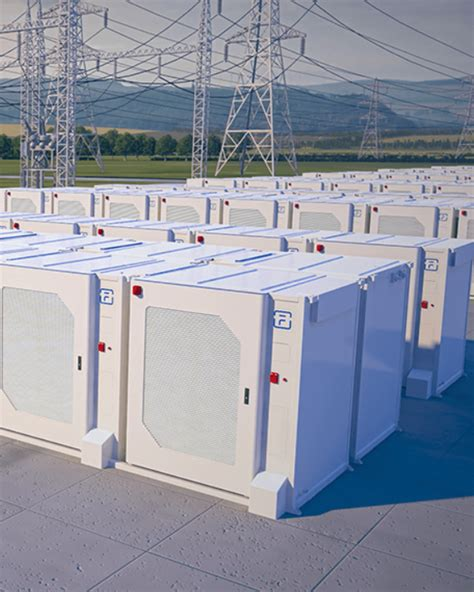
\includegraphics[width=80mm,scale=1]{energia_1.jpeg}
        \end{figure}
        Armazenamento de energia usando baterias.
    }

    \frame{
        \begin{figure}
          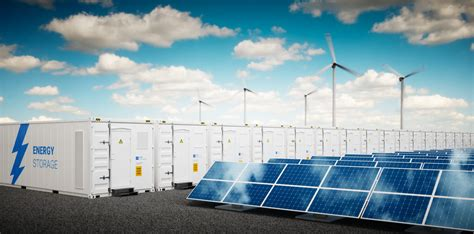
\includegraphics[width=80mm,scale=1]{energia_2.jpeg}
        \end{figure}
        Armazenamento de energia solar.
    }

    \frame {
        \frametitle{Projeto}
        \framesubtitle{Estrutura da proposta - Proposta - 2}
    \begin{itemize}
        \small
        \item Sugere-se a elaboração de um produto educacional, na forma de sequência didática acerca do temas das tecnologias de armazenamento de energia. Para tanto embasaremos tal conteúdo interdisciplinar nos conhecimentos reificados acerca das tecnologias de armazenamento de energia. O formato interdisciplinar exigido pelos itinerários formativos do Novo Ensino Médio moldará o produto considerando as habilidades e competências exigidas por este formato de ensino.
    \end{itemize}
    }

    \frame {
        \frametitle{Projeto}
        \framesubtitle{Estrutura da proposta - Metodologia - 1}
    \begin{itemize}
        \item Propõe-se uma investigação mista do conteúdo das representações sociais utilizando-se de ferramentas quantitativas de lingúistica computacional para construir um diagrama de Vergés, para se identificar o escopo da terminologia usada pelos discentes, ao explicarem as tecnologias de armazenamento de energia e seu impacto ambiental e societal. Para tanto somam-se estes aos procedimentos qualitativos das teorias de \citeonline{Representacees_sociais_moscovici} \citeonline{bardin_conteudo}.
    \end{itemize}
    }

    \frame {
        \frametitle{Projeto}
        \framesubtitle{Estrutura da proposta - Metodologia - 2}
    \begin{itemize}
        \footnotesize
        \item O prcedimento de coleta de dados e construção do corpus de texto analisado se dará no espaço do Colégio Instituto Estadual de Educação de Maringá, durante o período do segundo semestre do ano de 2022. Será utilizado um questionário aberto seguido de entrevista transcrita afim de se produzir o corpus de texto analisado onde serão questionados os estudantes, de maneira voluntária, anônima e não-avaliativa, discentes nos 1\textordmasculine, 2\textordmasculine e 3\textordmasculine anos do NEM regular e técnico, uma vez que estes, devido à transição para a nova grade curricular, já foram expostos à temas adjacentes ao conteúdo das representações estudadas nas matérias de física, química e biologia.
    \end{itemize}
    }

    \frame{
        \begin{figure}
          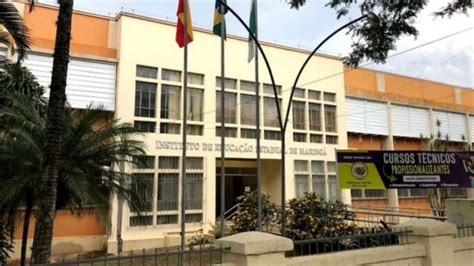
\includegraphics[width=80mm,scale=1]{ieem.jpeg}
        \end{figure}
        Fachada do Colégio Instituto.
    }

    \frame{
        \begin{figure}
          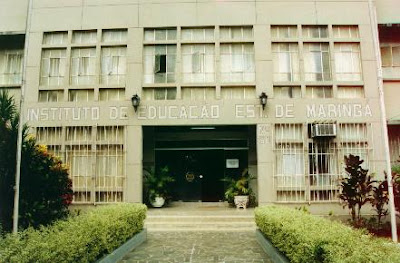
\includegraphics[width=80mm,scale=1]{ieem_2.jpeg}
        \end{figure}
        Fachada do Colégio Instituto.
    }

    \frame{
        \frametitle{Projeto}
        \framesubtitle{Estrutura da proposta - Hipótese e Resultados esperados}
    \begin{itemize}
        \item Quais as representações dos discentes acerca das tecnologias de de armazenamento de energia, seu impacto ambiental e societal.
        \item Espera-se encontrar uma significação pouco desenvolvida acerca das tecnologias de armazenamento de energia, seu impacto ambiental e societal.
    \end{itemize}
    }

    % \frame{
        % \frametitle{Cronograma}
        % \begin{tabular}{|c||l||r|}
           % { Procedimento & Início & Término \\ 
        % \hline
            % \makecell{Leitura e fichamento} & 2\textordmasculine sem. 2022 & 1\textordmasculine sem. 2022\\ 
        % \hline
            % \makecell{Coleta de dados} & 2\textordmasculine sem. 2022 & 1\textordmasculine sem. 2022\\
        % \hline
            % \makecell{Análise de dados} & 2\textordmasculine sem. 2022 & 2\textordmasculine sem. 2022\\
        % \hline
            % \makecell{Escrita final} & 2\textordmasculine sem. 2022 & 2\textordmasculine sem. 2022\\
        % \hline
        % \end{tabular}
    % }


\bibliography{interdisciplinaridade}
\end{document}
